%!TEX root = ../thesis.tex

%************************************************
\chapter{Dataset}\label{ch:data}
%************************************************

% Start with the pipes and some images of the pipelines and segments.

\section{Configuration}
\label{sec:dataset:configuration}

The data consisted of 24 CP areas. Each of these areas have one anode point where the current is pushed into the ground. The current is then propagated through the ground and led back to the anode through the steel gas pipes completing the electric system.

The pipes spread from the anode and branch off from each-other, creating a tree like structure. The pipes are divided into segments, Usually where a pipe branches into two pipelines, two new segments form. A pipe can only be part of one segment but a segment can consist of multiple pipes. In between the segments measuring points are placed to measure the current and difference in voltages in the segment. The number of segments an measuring points differ per area and is shown in table %todo ref table.

% show table with the number of measuring points and segments per area.
\begin{table}[!htb]
\label{tab:dataset:measuring-points-per-area}
    \begin{minipage}{.5\textwidth}
        \centering
        \caption{}
        \label{tab:first}
        \begin{tabular}{rcl}
            right & center & left \\
            right & center & left 
        \end{tabular}
    \end{minipage}%
    \begin{minipage}{.5\textwidth}
        \centering
        \caption{}
        \label{tab:second}
        \begin{tabular}{rcl}
            right & center & left \\
            right & center & left 
        \end{tabular}
    \end{minipage}
\end{table}

%mep uit!!!!

\section{Missing Data}
\label{sec:dataset:missing-data}
Usually the measurements are conducted once per year at every measuring point. The measurements started as early as 1987 up-until 2016. This means their should be 39 measurements per measuring point. However this is not the case as is shown in figure  %todo ref figure

\begin{figure}[!htb]
\centering
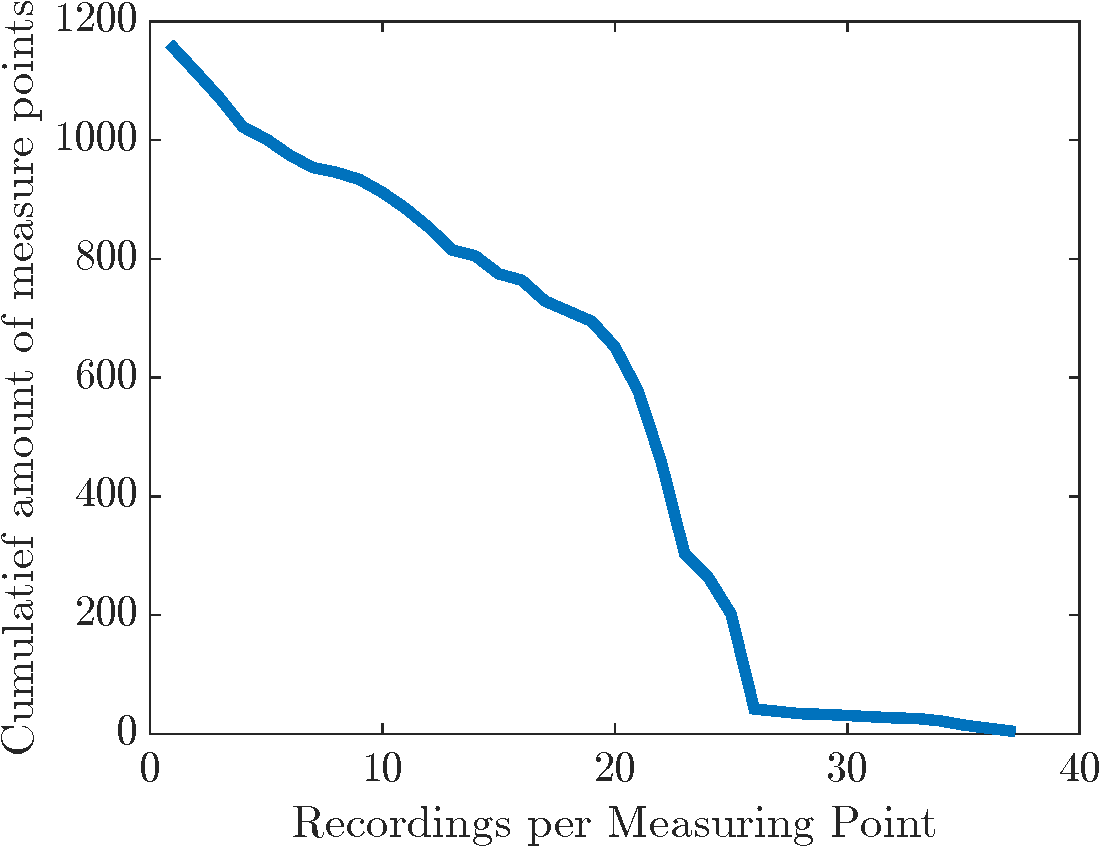
\includegraphics[width=.75\textwidth]{./gfx/chapters/data/cumulatief-recordings-per-measurepoint.pdf}
\caption{The number of measurements per measuring point against the cumulative number of measuring points having that number of measurements.}
\label{fig:dataset:cumulatief-recordings}
\end{figure}

Figure [REF] shows a fast drop in measurement points after the 20 measurements mark. At 26 measurements the drop stagnates and the maximum number of measurements is reached at 37 measurements. This means that none of the measuring points have the maximum number of 39 measurements.


% Tell about how the data was configured
% Show a figure with the tree, tell that it is a directed graph
% Tell about the different areas
% Tell about the measurepoints and that they have measurements

\section{Interpolation}
\label{sec:dataset:interpolation}
The method we proposed to use to predict the voltages of the pipelines with LVQ [REF] depends on the data being consistently spaced in time. 

Before the interpolation method was applied the data was checked for outliers by taking the mean and two times the standart deveation. Then removing the data points that did not fall in the range of $x > 2 \times \sigma - \mu$ and $x < 2 \times \sigma + \mu$.

\begin{figure}[!htb]
\centering
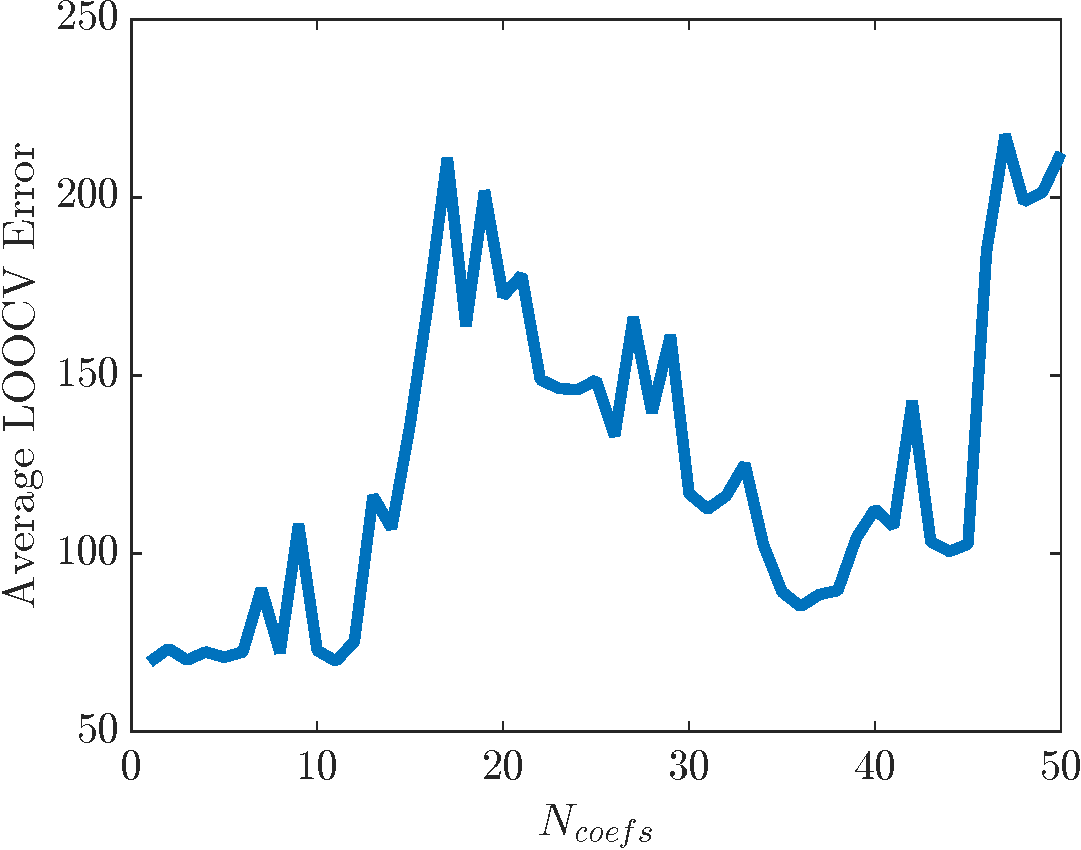
\includegraphics[width=.75\textwidth]{./gfx/chapters/data/Average-LOOCV-Error.pdf}
\caption{The average leave one out cross validation over all areas plotted against the number of $N$ coefficients used for the polynomial interpolation.}
\label{fig:dataset:cumulatief-recordings}
\end{figure}

% The data from the measuring points had many missing datapoints 
% The time (time-step) of the measurments was not concistent
% Used method to interpolate the data (show this in the method section)
% Describe the way this was done
% Leave One Out cross validation, to find an apropriate `n' (number of coeficients)
% Show the figure
% Describe the figure
% Tell the `n' should be 11 for reasons :D

